% PeerJ Computer Science submission manuscript; validated revision 2026-10-18
% Current source of record for the validated PeerJ revision.
% Conversion decisions only (no reframing of the science):
%   - Related Work folded into Introduction as a subsection (PeerJ Research
%     Article section order has no Related Work section).
%   - "Data and Method" -> "Materials & Methods".
%   - Threats to Validity and Limitations folded into Discussion as subsections.
%   - JAIR-specific reproducibility checklist appendix omitted; its substance
%     (data/code availability) is covered by the Data Availability statement.
%   - Unstructured abstract retained at the authors' request.
%   - Numeric citation style (PeerJ permits any full, clear, consistent style).
% 2026-10-16 PeerJ-compliance pass: Times font (mathptmx), Abstract on p.1 (no page break after cover page), references sorted Author/Year/Title, all figures/tables cited in text.
%   - Fixed an obvious duplicated word ("attached. attached.") in Conclusion.
\documentclass[12pt,letterpaper]{article}

\usepackage[margin=1in]{geometry}
\usepackage{lineno}
\usepackage{graphicx}
\usepackage{booktabs}
\usepackage{placeins}
\usepackage{amsmath,amssymb}
\usepackage[T1]{fontenc}
\usepackage{mathptmx} % PeerJ: 12pt Times font
\usepackage{hyperref}
\usepackage{xurl}
\hypersetup{hidelinks}
\usepackage[
  backend=bibtex,
  style=numeric,
  sorting=nyt, % PeerJ: reference list sorted by Author, Year, Title
  maxbibnames=99,
  minbibnames=99,
  giveninits=true
]{biblatex}
\addbibresource{refs.bib}

% PeerJ: figures cited as "Fig. 1" in text.
\renewcommand{\figurename}{Fig.}

% PeerJ: left-justified (ragged-right) body text.
\raggedright

\title{How Well Do Agent Failure Taxonomies Travel? A Cross-Dataset Empirical Analysis of Failure Labels in Public Agent Trajectory Datasets}

\author{}
\date{}

\begin{document}

% ================= AUTHOR COVER PAGE (PeerJ page 1) =================
\begin{center}
{\Large\bfseries How Well Do Agent Failure Taxonomies Travel? A Cross-Dataset Empirical Analysis of Failure Labels in Public Agent Trajectory Datasets\par}
\vspace{1.5em}

{\large Abhinav Tharamel Baiju\textsuperscript{1,*}, Tejaswini Viswanath\textsuperscript{2}\par}
\vspace{1em}

\textsuperscript{1}Independent Researcher, Chicago, Illinois, USA\\
% Affiliation wording ("Independent Researcher") still pending author confirmation; city confirmed Chicago (2026-10-16)
\textsuperscript{2}Independent Researcher, Chicago, Illinois, USA\\
% Affiliation wording ("Independent Researcher") still pending author confirmation; city confirmed Chicago (2026-10-16)
\vspace{1em}

\textsuperscript{*}Corresponding author: Abhinav Tharamel Baiju, \href{mailto:abhinavtb@gmail.com}{abhinavtb@gmail.com}\\
Tejaswini Viswanath: \href{mailto:tejaswiniviswanath@gmail.com}{tejaswiniviswanath@gmail.com}
\end{center}

% ================= END AUTHOR COVER PAGE =================
% PeerJ: Abstract follows on the same page (no page break after cover page).

\linenumbers

\begin{abstract}
The artificial intelligence (AI) agent-failure taxonomies examined here were developed using their authors' own trajectories, yet the field routinely treats these taxonomies as portable, universal descriptions of why agents fail. Whether failure categories mean the same thing or occur at comparable rates outside their home benchmark is essentially untested. We audit the portability assumption empirically: we map two independently produced public failure datasets to a single unified scheme and test whether the resulting failure-label distributions travel across datasets, domains, and models, while directly auditing the quality of the released labels. We annotate 384 agent failures, consisting of 200 AgentErrorBench trajectories (ALFWorld, GAIA, WebShop) and 184 Who\&When multi-agent failures, into a 13-class unified coding scheme defined for this audit, under a prospective analysis plan with prespecified hypotheses (H1--H3). Who\&When's free-text attributions were blind double-coded (agreement 69.6\%, Cohen's $\kappa=0.662$) with consensus adjudication; confirmatory tests use $\chi^2$ tests of independence with Cramer's $V$ and Monte Carlo permutation $p$-values. Harmonized label distributions differ dramatically across datasets ($\chi^2=160.48$, $df=12$, $p=4.2\times10^{-28}$, Cramer's $V=0.646$; H1 supported), across domains ($p=4.1\times10^{-23}$), and across models ($p=0.002$, $V=0.30$). H2 and H3 are not supported: coordination failures do not dominate the multi-agent data, and the empty-label rate is not established to exceed 15\%. A direct label-quality audit finds 13.5\% of AgentErrorBench annotations carry empty failure labels (concentrated in one model's trajectories), inconsistent category strings, and documentation mismatches. Because tasks, systems, and annotation protocols co-vary across the datasets, the gaps cannot isolate a taxonomy effect. Our results limit generalization of observed failure frequencies and show that label noise in public failure datasets is itself a first-order problem for the field. In these data, failure-label profiles are benchmark-, domain-, and model-relative. The distributional gaps limit generalization of the observed failure frequencies but cannot establish them on their own. We close with concrete recommendations for benchmark designers.
\end{abstract}

\section{Introduction}
The evaluation of large language model (LLM) agents has matured rapidly. Benchmarks now
span embodied control (ALFWorld~\cite{shridhar2021alfworld}), open-ended
assistant tasks (GAIA~\cite{mialon2024gaia}), web interaction
(WebShop~\cite{yao2022webshop}, WebArena~\cite{zhou2024webarena}), tool use
(API-Bank~\cite{li2023apibank}), software engineering
(SWE-agent~\cite{yang2024sweagent}), and general agentic competence
(AgentBench~\cite{liu2023agentbench}), and recent surveys systematize this
fast-moving evaluation landscape~\cite{yehudai2025survey}. In parallel, agent
\emph{architectures} have converged on a recognizable pattern: the
reason--act loop popularized by ReAct~\cite{yao2023react}, in which the model
interleaves chain-of-thought reasoning with tool calls, wrapped in scaffolding
for memory, planning and error handling.

Alongside the benchmarks, a parallel literature proposes \emph{taxonomies} of
agent failure: structured vocabularies (planning errors, tool errors,
grounding errors, and so on) intended to explain \emph{why} agents fail. These
taxonomies increasingly serve as the shared language of the field: papers
compare ``planning failures'' across systems, and debugging frameworks target
taxonomy categories as if they were stable, well-defined kinds.

The taxonomies examined here were developed using their authors' own
trajectories, in their own environments, with their own annotation protocols.
Whether the resulting categories mean the same thing, or even occur at
comparable rates, outside their home benchmark is essentially untested. If
failure labels do not travel across datasets, then cross-paper comparisons
built on them rest on sand, debugging tools tuned to one benchmark's failure
profile may misfire on the next, and the growing practice of treating
taxonomy categories as portable measurement
instruments~\cite{yehudai2025survey} is premature.

This paper presents a cross-dataset empirical analysis of that portability:
to our knowledge, the first to map two independently produced public
failure datasets to a single unified scheme and test the resulting
distributions. We take two
public, independently produced agent-failure datasets with incompatible native
labeling schemes and ask four prespecified research questions:

\begin{itemize}
\item \textbf{RQ1.} What is the distribution of failure labels within each dataset?
\item \textbf{RQ2.} After mapping to one unified scheme, which failure categories
dominate \emph{across} datasets, and which are dataset-specific?
\item \textbf{RQ3.} Do failure labels mean the same thing across datasets, and how
clean are the released labels themselves?
\item \textbf{RQ4.} Do failure distributions differ by agent domain (embodied, web,
general-assistant, multi-agent)?
\end{itemize}

We specified directional hypotheses in advance: (H1) label distributions differ
significantly across datasets; (H2) planning failures form the plurality in
web-navigation data while coordination failures dominate multi-agent data;
(H3) at least 15\% of native labels cannot be mapped without definitional
guesswork. H1 is strongly supported; H2 and H3 are not, and the ways in
which they fail are themselves informative. An additional exploratory analysis
(not prespecified) examines whether failure profiles differ across the
evaluated language models. We stress upfront that the two datasets differ
simultaneously in tasks, systems, and annotation protocols, so distributional
differences alone cannot isolate a taxonomy effect; we frame the study as a
descriptive audit of harmonized failure annotations and report the confounds
explicitly rather than claiming a controlled test of portability.

Our contributions are: (1) a cross-dataset quantitative analysis of
agent failure labels (384 annotated failures, two independently produced
datasets, four domains,
three models, one unified scheme); (2) evidence that harmonized
failure-label distributions are strongly dataset-, domain- and
model-dependent; (3) a
direct audit documenting label noise (empty labels, inconsistent strings,
documentation mismatches) in a published failure benchmark; (4) concrete
recommendations for benchmark designers; and (5) fully public data, mappings
and analysis code for reproduction.

\subsection{Related work}
\emph{Agent benchmarks.} ALFWorld~\cite{shridhar2021alfworld} aligns
text-based policies with embodied execution; GAIA~\cite{mialon2024gaia}
poses 466 real-world assistant questions requiring reasoning, multimodality
and tool use; WebShop~\cite{yao2022webshop} provides a large-scale simulated
e-commerce environment for grounded web agents; WebArena~\cite{zhou2024webarena}
extends web evaluation to 812 long-horizon tasks in self-hosted environments;
API-Bank~\cite{li2023apibank} targets tool-augmented LLMs with 73 APIs and
annotated dialogues; SWE-agent~\cite{yang2024sweagent} reframes software
engineering agents around the agent--computer interface; and
AgentBench~\cite{liu2023agentbench} evaluates 29 LLMs as agents across eight
interactive environments. \cite{yehudai2025survey}
survey the evaluation landscape. These benchmarks measure \emph{task
success}; they do not explain \emph{why} agents fail, which is the role
taxonomies claim.

\emph{Agent architectures.} ReAct~\cite{yao2023react} established the
reason--act trajectory structure that underlies most modern agents and,
consequently, most failure trajectories: a failure is almost always a
breakdown somewhere in an interleaved sequence of thoughts, actions and
observations. Our unified scheme's classes (planning, tool selection,
formatting, execution, observation reading) map directly onto positions in
this loop, which is why the scheme can serve as a common vocabulary at all.

\emph{More benchmarks, more failure surfaces.} The pattern (each benchmark
measuring success while leaving failure causes unlabeled) holds beyond our
two datasets. ALFRED~\cite{shridhar2020alfred} is the embodied
instruction-following benchmark on which ALFWorld is built; TPTU~\cite{ruan2023tptu}
benchmarks task planning and tool usage; TravelPlanner~\cite{xie2024travelplanner}
stresses multi-day travel planning with hard constraints; and
$\tau$-bench~\cite{yao2025taubench} evaluates tool--agent--user interaction in
realistic domains. Each would benefit from a portable failure vocabulary, and
each would likely exhibit the same dataset-specific label skew we document
here, since their task structures foreground different failure classes.

\emph{Learning from failures.} A parallel literature treats failure as
training signal rather than as object of study. Reflexion~\cite{shinn2023reflexion}
lets agents verbally reflect on failed trajectories and store the reflections
as episodic memory, improving subsequent attempts without weight updates; its
success depends entirely on correctly \emph{diagnosing} why a trajectory
failed. AgentPex~\cite{sharma2026agentpex} automatically detects failures in
agentic traces, a step toward scalable annotation. Both lines of work
presuppose what we test: that failure labels are reliable and comparable. Our
label-noise audit suggests that presupposition is shaky.

\emph{Failure taxonomies and debugging.} \cite{zhu2025agentdebug}
introduced the AgentErrorTaxonomy (error types across memory, reflection,
planning, action and system modules), the AgentErrorBench set of annotated
failure trajectories from ALFWorld, GAIA and WebShop, and the AgentDebug
three-stage debugging framework. \cite{zhang2025whowhen}
introduced Who\&When, a benchmark for automated failure attribution
in multi-agent systems: 184 annotated failures across algorithm-generated and
hand-crafted systems, each labeled with the responsible agent, the decisive
step, and a natural language explanation. \cite{cemri2025mast} introduced
MAST, a multi-agent failure taxonomy with MAST-Data: over 1,600 annotated
traces across seven multi-agent frameworks, including a human-annotated
subset (inter-annotator $\kappa{=}0.88$) and an LLM-as-judge annotation
pipeline. MAST is the closest existing multi-agent failure dataset to
Who\&When. We scope this paper to AgentErrorBench and Who\&When, the two
datasets whose per-trajectory failure labels were available in mappable form
when our prospective plan was frozen, and leave cross-walking MAST's
14-mode taxonomy into the unified scheme to future work; its human-annotated
subset would be a natural validation set. For this audit, we use an analyst-defined 13-class coding scheme as a common
vocabulary. Its operational definitions appear in Table~\ref{tab:classes};
the native-to-unified mappings and retrospective coding corrections are
released with the supplement. We do not claim that this scheme is a
validated universal taxonomy. Our contribution is the explicit harmonization
and quality audit of independently produced public annotations.

\section{Materials \& Methods}
Our analysis plan, hypotheses and mapping rules were fixed before
confirmatory statistics were computed (prospective analysis plan:
\texttt{PREREGISTRATION.md} in the supplement). The per-model
analysis in Section~\ref{sec:model} is exploratory and was not prespecified; we label
it as such.

\subsection{Datasets}
\label{sec:datasets}
\textbf{AgentErrorBench}~\cite{zhu2025agentdebug}: 200 annotated failure
trajectories: 100 ALFWorld (embodied), 50 GAIA (general assistant), 50
WebShop (web navigation), produced by three models (GPT-4o: 81, Qwen3-8B:
62, Llama3.3-70B-Turbo: 57). Each trajectory carries one step annotation: a
module key and a \texttt{failure\_type} drawn from the AgentErrorTaxonomy,
plus a free-text reasoning string. (The taxonomy's documentation is itself
inconsistent: the README claims 17 error types, while the released
definition file contains 18 distinct label strings across 19
module-qualified pairs; see Section~\ref{sec:rq3}.) We use the released label files
(\texttt{alfworld\_labels.json}, \texttt{gaia\_labels.json},
\texttt{webshop\_labels.json}) verbatim.

\textbf{Who\&When}~\cite{zhang2025whowhen}: 184 annotated multi-agent
failures (126 algorithm-generated, 58 hand-crafted systems such as
Magnetic-One). Each record gives the responsible agent
(\texttt{mistake\_agent}), the decisive step, and a free-text
\texttt{mistake\_reason}. Only 4 of 184 records carry a structured
\texttt{mistake\_type}; the rest are free text. The 184 rows cover 139
unique questions; 45 questions contribute a second row.

The API-Bank dialogue corpus~\cite{li2023apibank} was examined as a third
candidate source but excluded: it contains API documentation and simulated
exception strings but no failure annotations, so it cannot be mapped to the
unified scheme without inventing labels. It is discussed qualitatively only.

\subsection{Unified scheme and mapping}
\label{sec:mapping}
Representative native mappings are shown in Table~\ref{tab:mapping}.
We map both datasets to our 13-class unified scheme (defined in
Table~\ref{tab:classes}):
\texttt{PLAN}, \texttt{TOOL\_SELECT}, \texttt{TOOL\_FORMAT},
\texttt{TOOL\_EXEC}, \texttt{OBS\_MISREAD}, \texttt{GROUNDING},
\texttt{NO\_RECOVERY}, \texttt{LOOP}, \texttt{GIVE\_UP},
\texttt{VERIFICATION}, \texttt{MEMORY}, \texttt{COORDINATION},
\texttt{OTHER}. AgentErrorBench's native types map deterministically via
published definitions. System-level resource exhaustion (\texttt{step\_limit}) has no
unified counterpart and maps to \texttt{OTHER}, exposing a scheme gap we
report rather than hide. Who\&When's free-text reasons were coded by the
author into the same scheme under a documented coding guide (e.g., ``code is
incorrect'' $\rightarrow$ \texttt{UNMAPPABLE} (no malformed argument, schema violation, or unparseable call stated); ``fabricated the population
figures'' $\rightarrow$ \texttt{GROUNDING}; ``did not verify \ldots
assumptions'' $\rightarrow$ \texttt{VERIFICATION}). To measure coding
reliability, the second author independently blind-coded all 184 Who\&When
rows against the original codebook (no access to the first coder's labels).
Inter-annotator agreement was 69.6\% (128/184), Cohen's $\kappa=0.662$
(substantial). Disagreements concentrated on 34 rows where the second coder
judged vague reasons unmappable (\texttt{UNMAPPABLE}), 27 of them bare
``code is incorrect'' reasons the coding guide had mapped to \texttt{TOOL\_FORMAT}.
Applying the Table~\ref{tab:classes} definition of \texttt{TOOL\_FORMAT}
(malformed arguments, schema violations, unparseable calls), those 27 rows
are coded \texttt{UNMAPPABLE} in the consensus (Section~\ref{sec:robustness}).
All 56 disagreements (30\% of rows) were adjudicated to consensus labels; in the final consensus, 4 resolve to the first
coder's label, 51 to the second's, 1 to a third reading; all analyses use these retrospectively corrected labels. The original
consensus labels and notes are preserved alongside the revised labels;
this correction is not a new independent human annotation round. Coder-specific distributions and sensitivity analyses of
the contested mappings are reported in Section~\ref{sec:robustness}, which shows which
findings depend on the disputed decisions and which survive them.
All 184 codings with rationales are
released. Records that cannot be mapped without guessing are coded
\texttt{UNMAPPABLE} and reported, never silently dropped.

\begin{table}[t]
\centering
\caption{Representative native-to-unified mappings (full table released).}
\label{tab:mapping}
\begin{tabular}{@{}lll@{}}
\toprule
Native label & Unified & Basis \\
\midrule
\texttt{planning.inefficient\_plan} & \texttt{PLAN} & direct \\
\texttt{planning.constraint\_ignorance} & \texttt{PLAN} & direct \\
\texttt{reflection.progress\_misjudge} & \texttt{OBS\_MISREAD} & direct \\
\texttt{reflection.causal\_misattribution} & \texttt{OBS\_MISREAD} & direct \\
\texttt{memory.over\_simplification} & \texttt{MEMORY} & direct \\
\texttt{reflection.hallucination} & \texttt{MEMORY} & definition-based$^*$ \\
\texttt{action.parameter\_error} & \texttt{TOOL\_FORMAT} & direct \\
\texttt{system.tool\_execution\_error} & \texttt{TOOL\_EXEC} & direct \\
\texttt{system.step\_limit} & \texttt{OTHER} & scheme gap \\
\texttt{action.misalignment} & \texttt{TOOL\_SELECT} & direct \\
\bottomrule
\end{tabular}
\begin{flushleft}\footnotesize{$^*$Module says reflection, but the published
definition (``believes it performed actions that never occurred'') describes
false recall, a memory phenomenon.}\end{flushleft}
\end{table}

\begin{table}[t]
\centering
\caption{The 13 unified failure classes (our frozen scheme),
with definitions and illustrative examples. No released annotation mapped to
\texttt{NO\_RECOVERY} under our coding procedure.}
\label{tab:classes}
\begin{tabular}{@{}l p{0.38\textwidth} p{0.38\textwidth}@{}}
\toprule
Class & Definition & Example \\
\midrule
\texttt{PLAN} & Wrong decomposition, incoherent strategy, goal misunderstanding &
  agent pursues steps in an impossible order \\
\texttt{TOOL\_SELECT} & Wrong tool/API chosen for a reasonable sub-goal &
  web search called for arithmetic needing a calculator \\
\texttt{TOOL\_FORMAT} & Malformed arguments, schema violations, unparseable calls &
  JSON missing a required field; wrong parameter type \\
\texttt{TOOL\_EXEC} & The tool itself fails: crashes, timeouts, auth failures &
  API timeout; environment crashes mid-episode \\
\texttt{OBS\_MISREAD} & Correct observation, wrong inference drawn from it &
  ``item out of stock'' read as purchase success \\
\texttt{GROUNDING} & Hallucinated or unsupported observations cited as evidence &
  quotes a price appearing nowhere on the page \\
\texttt{NO\_RECOVERY} & Informative error followed by verbatim retry or
  abandonment without trying an alternative & resubmits the identical
  call after ``invalid date format'' \\
\texttt{LOOP} & Repeated near-identical actions with no forward progress &
  same search query issued five times in a row \\
\texttt{GIVE\_UP} & Premature termination; false infeasibility claim &
  declares the task impossible after one failed attempt \\
\texttt{VERIFICATION} & Skipped or incorrect verification before acting/answering &
  final answer submitted without checking it \\
\texttt{MEMORY} & False recall, omission, forgetting, history errors &
  forgets a constraint stated three turns earlier \\
\texttt{COORDINATION} & Multi-agent only: role disobedience, inter-agent
  misalignment, false consensus & executor ignores the planner's revised plan \\
\texttt{OTHER} & Residual: named category fitting none of the above &
  disallowed content; corrupt task inputs \\
\bottomrule
\end{tabular}
\end{table}

\subsection{Statistics}
\label{sec:stats}
Per-dataset proportions use 95\% Wilson confidence intervals. H1, the domain
comparison (RQ4) and the exploratory model comparison use $\chi^2$ tests of
independence ($\alpha{=}0.05$) with standardized residuals; effect size via
Cramer's $V$. Because several expected cell counts fall below five, we
additionally computed Monte Carlo permutation $p$-values (100{,}000 uniform
label permutations per test, seed 7, Pearson $\chi^2$ statistic, group sizes
fixed). Exceedance counts: H1 $0/100{,}000$; domain $0/100{,}000$; model
$195/100{,}000$ ($p{=}0.0020$). Conclusions were unchanged at
$\alpha{=}0.05$. (An earlier version of the permutation script contained a
vectorization bug that pooled permutations before tabulating, understating
$p$; the corrected implementation was verified against an independent
plain-loop reimplementation, and we report the corrected figures
throughout.) Residuals are used descriptively to localize each omnibus
association; individual cells are not treated as separately confirmatory
tests. H2 compares the plurality class per domain; H3 is a one-sided
proportion check. Deviation from the prospective plan: the plan listed
Jensen-Shannon divergence between conditional sub-label distributions as
part of the RQ3 label-shift audit; it was not computed because the datasets
do not provide comparable shared sub-label distributions, so RQ3 was
evaluated through definition comparison and the label-quality audit instead.
Second deviation: the frozen coding guide mapped bare ``code is incorrect''
reasons to \texttt{TOOL\_FORMAT}; applying the Table~\ref{tab:classes} class
definition, 27 such rows were recoded \texttt{UNMAPPABLE}
(Section~\ref{sec:robustness}). The hypotheses and confirmatory tests are unchanged.

\section{Results}
We report the confirmatory results for RQ1--RQ4 and the prespecified hypotheses H1--H3, followed by the exploratory model comparison (Section~\ref{sec:model}), robustness and sensitivity analyses (Section~\ref{sec:robustness}), and domain narratives from the residuals (Section~\ref{sec:narratives}).

\subsection{RQ1: Within-dataset distributions}
\label{sec:rq1}
AgentErrorBench ($n{=}200$) is dominated by \texttt{PLAN} (69; 34.5\%, 95\%
CI 28.3--41.3\%), followed by \texttt{OBS\_MISREAD} (37; 18.5\%) and
\texttt{MEMORY} (35; 17.5\%). \texttt{TOOL\_EXEC} (6.0\%),
\texttt{OTHER} (4.0\%), \texttt{TOOL\_SELECT} (3.5\%) and
\texttt{TOOL\_FORMAT} (2.5\%) are rare; 27 records (13.5\%, CI 9.4--18.9\%)
are \texttt{UNMAPPABLE}. Who\&When ($n{=}184$) shows a markedly different
profile: among mapped classes, \texttt{GROUNDING} (36; 19.6\%, CI 14.5--25.9\%) leads, then
\texttt{VERIFICATION} (28; 15.2\%, CI 10.7--21.1\%), \texttt{PLAN} (20;
10.9\%, CI 7.1--16.2\%), \texttt{TOOL\_EXEC} (15; 8.2\%),
\texttt{TOOL\_FORMAT} (10; 5.4\%, CI 3.0--9.7\%) and \texttt{OTHER} (10; 5.4\%),
\texttt{TOOL\_SELECT} (8; 4.3\%), \texttt{OBS\_MISREAD} (7; 3.8\%),
\texttt{COORDINATION} (6; 3.3\%), \texttt{LOOP} (5; 2.7\%),
\texttt{GIVE\_UP} (3; 1.6\%) and \texttt{MEMORY} (1; 0.5\%). A further 35 records
(19.0\%, CI 14.0--25.3\%) are \texttt{UNMAPPABLE}. Notably,
no released annotation in either dataset mapped to
\texttt{NO\_RECOVERY}, and
\texttt{MEMORY} is prevalent in AgentErrorBench but appears only once in
Who\&When, while
\texttt{VERIFICATION}, \texttt{GROUNDING}, \texttt{LOOP},
\texttt{GIVE\_UP} and \texttt{COORDINATION} appear only in Who\&When (Fig.~\ref{fig:dataset}).

\begin{figure}[htbp]
\centering
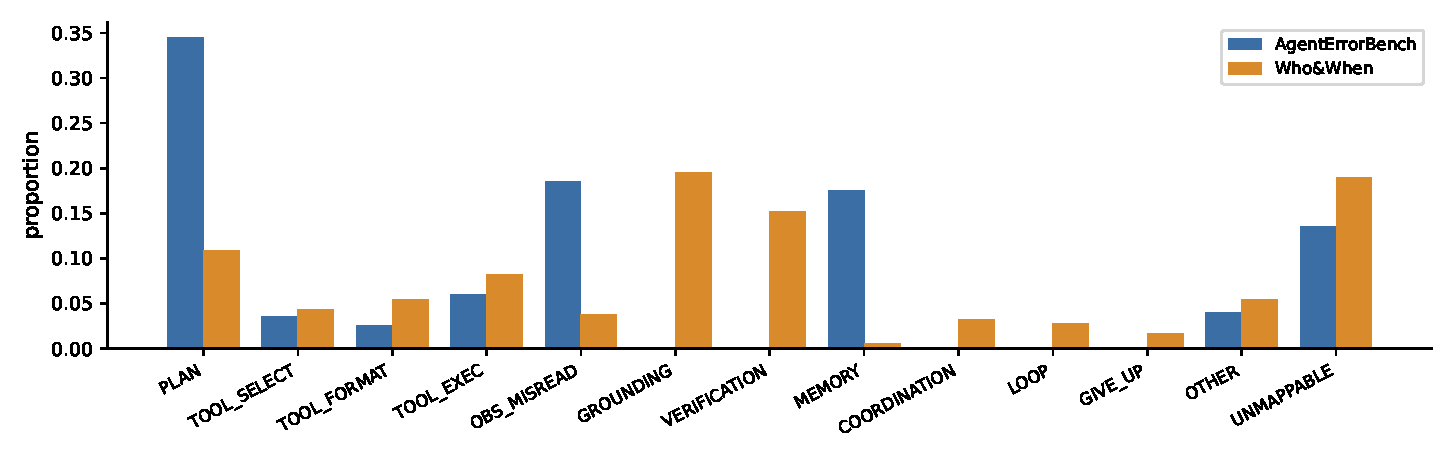
\includegraphics[width=0.95\linewidth]{figures/Figure1.pdf}
\caption{Unified failure-class distribution by dataset. Percentages use all released rows within each dataset.}
\label{fig:dataset}
\end{figure}

\subsection{RQ2/H1: Cross-dataset comparison}
\label{sec:rq2}
The distributions differ overwhelmingly: $\chi^2{=}160.48$, $df{=}12$,
$p{=}4.2\times10^{-28}$, Cramer's $V{=}0.646$ (permutation $p{\approx}10^{-5}$, $0/100{,}000$
exceedances; \textbf{H1 supported}). Standardized residuals
($|r|{>}2$) show AgentErrorBench over-representing \texttt{PLAN} ($r{=}+3.33$),
\texttt{OBS\_MISREAD} ($+2.94$) and \texttt{MEMORY} ($+3.75$), while Who\&When over-represents
\texttt{GROUNDING} ($+4.51$) and
\texttt{VERIFICATION} ($+3.98$). Excluding \texttt{UNMAPPABLE} as a robustness check leaves
the conclusion unchanged ($\chi^2{=}158.93$, $df{=}11$,
$p{=}2.2\times10^{-28}$, Cramer's $V{=}0.703$, a very large effect). In plain terms: the observed distributions are strongly
associated with dataset membership, so aggregate failure frequencies should not
be generalized across these datasets.

\subsection{RQ3: Do labels mean the same thing? Label-noise audit}
\label{sec:rq3}
Two findings. First, a qualitative comparison of AgentErrorTaxonomy's
published definitions against our unified classes reveals genuine
incommensurability at the margins: e.g., reflection-module
\texttt{hallucination} (``believes it performed actions that never
occurred'') is a memory phenomenon wearing a reflection label
(Table~\ref{tab:mapping}), and \texttt{step\_limit} (resource exhaustion)
has no counterpart in the unified scheme at all.

Second, the released AgentErrorBench labels are noisy \emph{in themselves}:
27 of 200 annotations (13.5\%) carry an \textbf{empty}
\texttt{failure\_type} with empty reasoning, unmappable without guessing.
The empties are not random: 24 of 57 Llama3.3-70B-Turbo trajectories (42.1\%)
are empty versus 3 of 62 Qwen3-8B (4.8\%) and 0 of 81 GPT-4o (0\%; see
Fig.~\ref{fig:empty}), suggesting a systematic annotation-pipeline gap for
one model. The files additionally contain inconsistent category strings
requiring normalization before any analysis (Fig.~\ref{fig:native} shows the
raw label distribution):
\texttt{plan\_inefficient} vs.\ \texttt{inefficient\_plan},
\texttt{Parameter\_error} vs.\ \texttt{parameter\_error}, a trailing-space
variant of \texttt{tool\_execution\_error}, and a \texttt{plan} vs.\
\texttt{planning} module-key split between WebShop and GAIA files. Even the
taxonomy's size is inconsistently documented: the README claims 17 error
types, but \texttt{error\_definitions.py} defines 18 distinct label strings
(19 module-qualified pairs). Any secondary analysis that naively counts
native labels will therefore undercount or split categories.
Table~\ref{tab:variants} lists every normalization our curation applied; we
recommend benchmark releases ship such a table themselves rather than leaving
it to secondary analysts to discover.

\begin{table}[t]
\centering\small
\caption{Label-string normalizations applied during curation. The first three
variants were attested in the repository's definition files; the module-key
split was attested in the released data files. In the data files the
normalized \texttt{planning.inefficient\_plan} form accounts for 46 of 200
records.}
\label{tab:variants}
\begin{tabular}{@{}ll@{}}
\toprule
Normalization & Attested in \\
\midrule
\texttt{plan\_inefficient} $\rightarrow$ \texttt{inefficient\_plan} & definition files \\
\texttt{Parameter\_error} $\rightarrow$ \texttt{parameter\_error} & definition files \\
trailing space after \texttt{tool\_execution\_error} & definition files \\
\texttt{plan.*} $\rightarrow$ \texttt{planning.*} (module key) & data files \\
\bottomrule
\end{tabular}
\end{table}

\begin{figure}[t]
\begin{minipage}{0.48\linewidth}
\centering
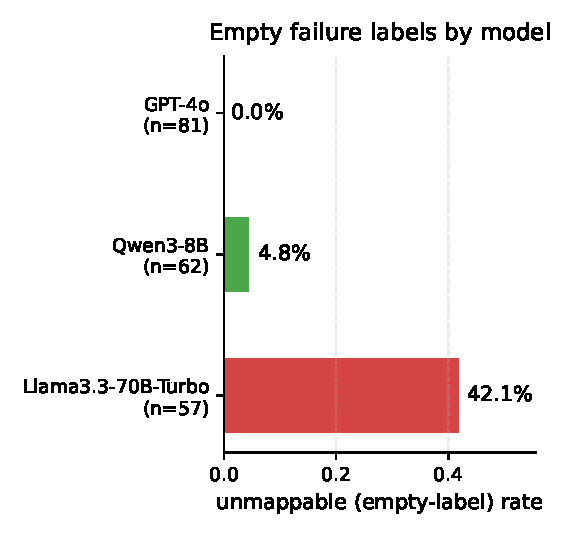
\includegraphics[width=\linewidth]{figures/Figure2.pdf}
\caption{Unmappable (empty) label rate by model in AgentErrorBench. The
noise is concentrated in one model's trajectories.}
\label{fig:empty}
\end{minipage}\hfill
\begin{minipage}{0.48\linewidth}
\centering
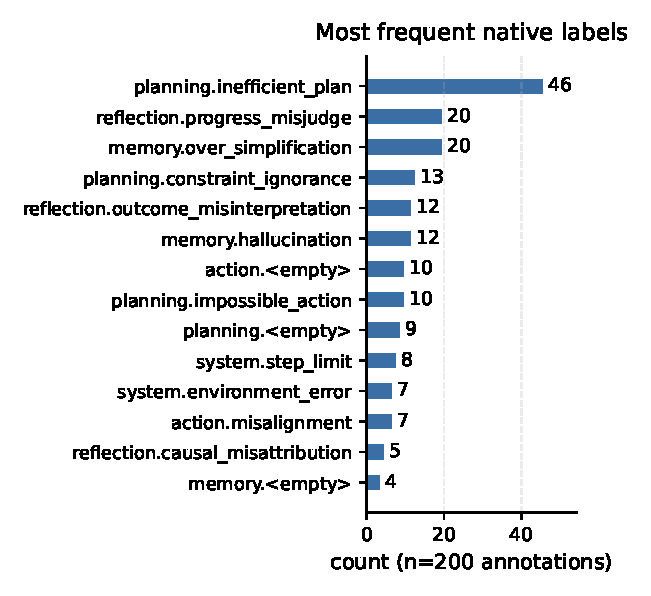
\includegraphics[width=\linewidth]{figures/Figure3.pdf}
\caption{Most frequent native failure labels in AgentErrorBench after
label-string normalization, before unified mapping ($n{=}200$).}
\label{fig:native}
\end{minipage}
\end{figure}

\subsection{RQ4/H2/H3: Domains and hypotheses}
\label{sec:rq4}
Failure profiles differ significantly by domain ($\chi^2{=}185.29$,
$df{=}33$, $p{=}4.1\times10^{-23}$, permutation $p{\approx}10^{-5}$
($0/100{,}000$ exceedances)). This test excludes the 62 \texttt{UNMAPPABLE}
records and the all-zero \texttt{NO\_RECOVERY} class.
Plurality classes: WebShop
\texttt{PLAN} (19/49, 38.8\%), ALFWorld \texttt{PLAN} (24/74, 32.4\%), GAIA
\texttt{PLAN} (26/50, 52.0\%), multi-agent \texttt{GROUNDING} (36/184 records
overall, 19.6\%; 36/149 mapped records, 24.2\%). \textbf{H2 is not supported}: while planning failures do form the
plurality in web navigation as predicted, coordination failures do
\emph{not} dominate the multi-agent data (3.3\%, ninth of twelve mapped classes).
Multi-agent failures in Who\&When are instead dominated by fabricated
information and unchecked outputs: individual-agent competence failures, not interaction
failures. A further 35/184 (19.0\%) multi-agent reasons are \texttt{UNMAPPABLE}
under the corrected coding rule (Section~\ref{sec:robustness}). \textbf{H3 is not supported}:
an exact one-sided binomial test of $H_0{:}\;p{\leq}0.15$ against
$H_1{:}\;p{>}0.15$ on the 27/200 empty native labels gives $p{=}0.75$.
(H3 uses AgentErrorBench alone: its \texttt{UNMAPPABLE} records are empty
native failure\_type fields, a property of the released labels, whereas
Who\&When carries no native labels at all, so the construct is not
comparable across datasets.)
Table~\ref{tab:contingency} gives the full contingency table, shown visually in Fig.~\ref{fig:domain}.

\begin{table}[t]
\centering
\caption{Unified failure-class counts by domain (row: class; columns:
embodied, web, general-assistant, multi-agent).}
\label{tab:contingency}
\begin{tabular}{@{}lrrrr@{}}
\toprule
Class & ALFWorld & WebShop & GAIA & Multi-agent \\
& ($n{=}100$) & ($n{=}50$) & ($n{=}50$) & ($n{=}184$) \\
\midrule
\texttt{PLAN} & 24 & 19 & 26 & 20 \\
\texttt{OBS\_MISREAD} & 19 & 9 & 9 & 7 \\
\texttt{MEMORY} & 16 & 14 & 5 & 1 \\
\texttt{TOOL\_EXEC} & 3 & 5 & 4 & 15 \\
\texttt{TOOL\_FORMAT} & 1 & 1 & 3 & 10 \\
\texttt{TOOL\_SELECT} & 3 & 1 & 3 & 8 \\
\texttt{GROUNDING} & 0 & 0 & 0 & 36 \\
\texttt{VERIFICATION} & 0 & 0 & 0 & 28 \\
\texttt{COORDINATION} & 0 & 0 & 0 & 6 \\
\texttt{OTHER} & 8 & 0 & 0 & 10 \\
\texttt{GIVE\_UP} & 0 & 0 & 0 & 3 \\
\texttt{LOOP} & 0 & 0 & 0 & 5 \\
\texttt{NO\_RECOVERY} & 0 & 0 & 0 & 0 \\
\texttt{UNMAPPABLE} & 26 & 1 & 0 & 35 \\
\bottomrule
\end{tabular}
\end{table}

\begin{figure}[htbp]
\begin{minipage}{0.48\linewidth}
\centering
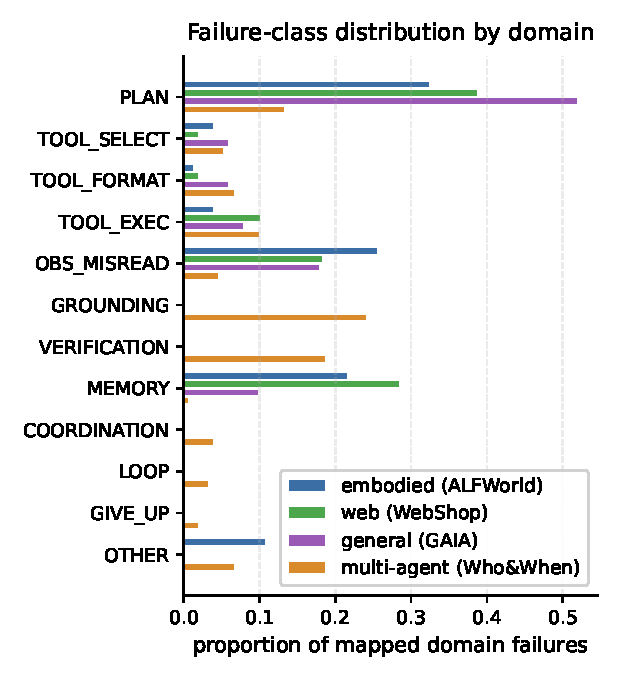
\includegraphics[width=\linewidth]{figures/Figure4.pdf}
\caption{Unified failure-class distribution by domain among mapped records (embodied, web,
general-assistant, multi-agent).}
\label{fig:domain}
\end{minipage}\hfill
\begin{minipage}{0.48\linewidth}
\centering
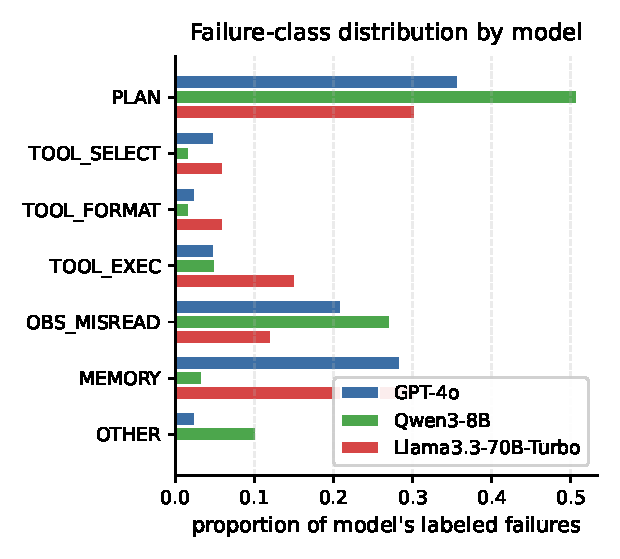
\includegraphics[width=\linewidth]{figures/Figure5.pdf}
\caption{Unified failure-class distribution by model (AgentErrorBench,
labeled records only).}
\label{fig:model}
\end{minipage}
\end{figure}

\subsection{Exploratory: failure profiles differ by model}
\label{sec:model}
Within AgentErrorBench, the three evaluated models show significantly
different failure profiles ($\chi^2{=}30.72$, $df{=}12$, $p{=}0.002$,
permutation $p{=}0.0020$ ($195/100{,}000$ exceedances),
Cramer's $V{=}0.30$, excluding unmappable records). GPT-4o's labeled failures
concentrate in \texttt{PLAN} (29/81), \texttt{MEMORY} (23/81) and
\texttt{OBS\_MISREAD} (17/81); Qwen3-8B is strikingly plan-heavy
(\texttt{PLAN} 30/59 labeled, 50.8\%) with \texttt{MEMORY} significantly
under-represented ($r{=}-2.88$); Llama3.3-70B-Turbo's 33 labeled failures
spread across \texttt{PLAN} (10), \texttt{MEMORY} (10) and
\texttt{TOOL\_EXEC} (5). Models differ in domain composition, so the pooled
comparison could in principle reflect domain mix rather than model:
GPT-4o's trajectories are 50/81 ALFWorld, versus 23/57 for
Llama3.3-70B-Turbo and 27/62 for Qwen3-8B. The model effect survives
holding domain fixed: permuting model labels within domains leaves the
pooled association significant (stratified permutation $p{=}0.0032$,
20,000 permutations), and within the single largest shared domain,
ALFWorld ($n{=}74$ labeled), GPT-4o and Qwen3-8B still differ sharply
($\chi^2{=}21.23$, $df{=}6$, $p{=}0.0017$, Cramer's $V{=}0.54$; Qwen
records no \texttt{MEMORY} failures in ALFWorld, 0/24, versus 16/50 for
GPT-4o). Llama3.3-70B-Turbo contributes no labeled ALFWorld trajectories
at all (all 23 empty), so it drops out of that within-domain check.
In other words, among available labeled
trajectories, failure profiles differed across models: even holding the
benchmark fixed, \emph{which model} failed predicts \emph{how} it failed.
This comparison is distorted by non-random missingness, however: with 42.1\%
of Llama3.3-70B-Turbo's annotations empty versus 0\% for GPT-4o, the labeled
Llama trajectories may not represent that model's full failure profile, so
the model-level result should be read as exploratory. The observed frequencies vary across these models (Fig.~\ref{fig:model}),
but this does not establish a failure mechanism or taxonomy measurement
invariance across models.


\subsection{Robustness: coder-specific distributions and sensitivity analyses}
\label{sec:robustness}
The Who\&When coding hinged on one consequential boundary decision: the
original coding guide mapped bare ``code is incorrect'' reasons to \texttt{TOOL\_FORMAT}
(produced artifact malformed), while the second coder judged 34 explanations
too vague to map at all (\texttt{UNMAPPABLE}). Of the 56 independent
disagreements, 27 were coder-1-\texttt{TOOL\_FORMAT} versus
coder-2-\texttt{UNMAPPABLE}. The two coders' distributions differ
accordingly: coder 1: \texttt{TOOL\_FORMAT} 40 (21.7\%), \texttt{GROUNDING}
38 (20.7\%), \texttt{PLAN} 23 (12.5\%); coder 2: \texttt{GROUNDING} 37
(20.1\%), \texttt{UNMAPPABLE} 34 (18.5\%), \texttt{VERIFICATION} 29 (15.8\%),
\texttt{TOOL\_FORMAT} 9 (4.9\%), but agree on the classes they
\emph{don't} dispute: \texttt{GROUNDING}, \texttt{VERIFICATION} and
\texttt{PLAN} appear at similar ranks in both.

We retrospectively revised the boundary by applying the Table~\ref{tab:classes} definition of
\texttt{TOOL\_FORMAT} as written (malformed arguments, schema violations,
unparseable calls): a reason is coded \texttt{TOOL\_FORMAT} only if it
describes a defect in the form of a call or its arguments. Bare ``code is
incorrect'' reasons, and reasons describing logic defects or outcomes (wrong
results, no output, unhandled edge cases) without a defect in the call's
form, are coded \texttt{UNMAPPABLE}. This recodes 27 consensus rows from
\texttt{TOOL\_FORMAT} to \texttt{UNMAPPABLE} (listed with rationales in the
released coding table); the recoded set coincides exactly with the 27 coder-1-\texttt{TOOL\_FORMAT}
versus coder-2-\texttt{UNMAPPABLE} disagreements, not with all 34
second-coder unmappable rows. Ten retained \texttt{TOOL\_FORMAT} labels use a broader operational
interpretation, including placeholder values, missing imports, nonexistent
columns and inadequate search queries. Some describe semantic or
implementation problems rather than a demonstrated schema or parsing
failure. We therefore also report a strict sensitivity analysis that recodes
all ten as \texttt{UNMAPPABLE}; the dataset association persists
($\chi^2{=}167.29$, $df{=}12$, $p{=}1.7\times10^{-29}$,
$V{=}0.660$). Grounding remains the largest mapped class, while the
unmappable share rises to 45/184 (24.5\%). This exposes a remaining
construct boundary rather than resolving it by assumption.
The consensus Who\&When distribution is now
\texttt{GROUNDING} 36 (19.6\%), \texttt{VERIFICATION} 28 (15.2\%),
\texttt{PLAN} 20 (10.9\%), \texttt{TOOL\_FORMAT} 10 (5.4\%).

As a remaining sensitivity check, we re-ran the headline tests using all
second-coder labels instead of the consensus: the omnibus H1 test is
essentially unchanged ($\chi^2{=}157.41$, $df{=}12$,
$p{=}1.8\times10^{-27}$, $V{=}0.640$, vs.\ consensus $\chi^2{=}160.48$,
$V{=}0.646$), as is the domain comparison
($\chi^2{=}183.15$ vs.\ $185.29$), and the Who\&When top class remains
\texttt{GROUNDING} (37/184). The cross-dataset distributional gap and the
grounding plurality are therefore robust to the remaining coder
disagreement; the earlier tool-formatting plurality is absent from the revised
consensus and coder 2, although it remains present in coder 1.

\subsection{Cluster-aware sensitivity: question-level dependence}
\label{sec:cluster}
Who\&When contributes 184 rows from 139 unique questions, with 45 questions
contributing two rows. We added a retrospective sensitivity analysis that
keeps each question intact. AgentErrorBench's 200 released trajectory IDs
are unique; shared underlying task IDs cannot be established from these
labels, so residual dependence between its trajectories remains possible.
For the dataset comparison there are 339 clusters; after removing
unmappable rows the domain comparison has 286 nonempty clusters.

We permuted group labels within cluster-size strata, preserving the number
of clusters per group and the observed multiplicities. Two-row questions
occur only in Who\&When and therefore do not exchange dataset labels with
singleton trajectories. Using Pearson's statistic, seed 7 and 20,000
permutations, both associations have zero exceedances; the plus-one Monte
Carlo estimate is $p{=}1/20{,}001\approx5\times10^{-5}$. These conditional
reference tests assume exchangeability within size strata and are not
causal tests of taxonomy effects.

Resampling the 139 Who\&When questions with replacement 20,000 times
(seed 7) yields row-weighted grounding 19.6\% (percentile 95\% CI
14.1--25.3\%) and coordination 3.3\% (CI 1.1--6.0\%). Grounding is a
plurality among mapped classes in 86.7\% of samples when ties count,
and the unique plurality in 83.5\%. These intervals capture empirical
question-level sampling variation, not coding uncertainty or population
representativeness. The full procedure and outputs are released.

\subsection{Domain narratives: what the residuals say}
\label{sec:narratives}
Standardized residuals by domain (Fig.~\ref{fig:residuals}) turn the
contingency table into four interpretable stories. \emph{Embodied
(ALFWorld)} failures over-represent observation misreading ($r{=}+2.8$) and
memory lapses ($+2.7$) while under-representing grounding ($-2.9$) and verification ($-2.5$): the released annotations emphasize observation interpretation and memory.
These frequencies do not independently establish causal mechanisms. \emph{General-assistant (GAIA)} failures are plan-dominated ($+3.3$)
with grounding ($-2.4$) and verification ($-2.1$) under-represented: the released general-assistant annotations emphasize planning. \emph{Web (WebShop)} failures over-represent
memory ($+3.6$) while under-representing grounding ($-2.3$) and verification ($-2.1$): the released web annotations emphasize memory and constraints; we did not
experimentally compare debugging interventions.
\emph{Multi-agent (Who\&When)} is the mirror image: grounding ($+4.7$) and
verification ($+4.2$) are over-represented while
memory ($-3.8$), planning ($-3.3$) and observation misreading ($-3.0$) are
under-represented. Strikingly, \texttt{COORDINATION} never rises above a
minority class in any domain; under the consensus coding, the multi-agent annotations emphasize individual-agent content and
verification problems more often than explicit coordination labels. Each domain's profile
is coherent on its own terms; none of them is the universal profile.

\begin{figure}[htbp]
\centering
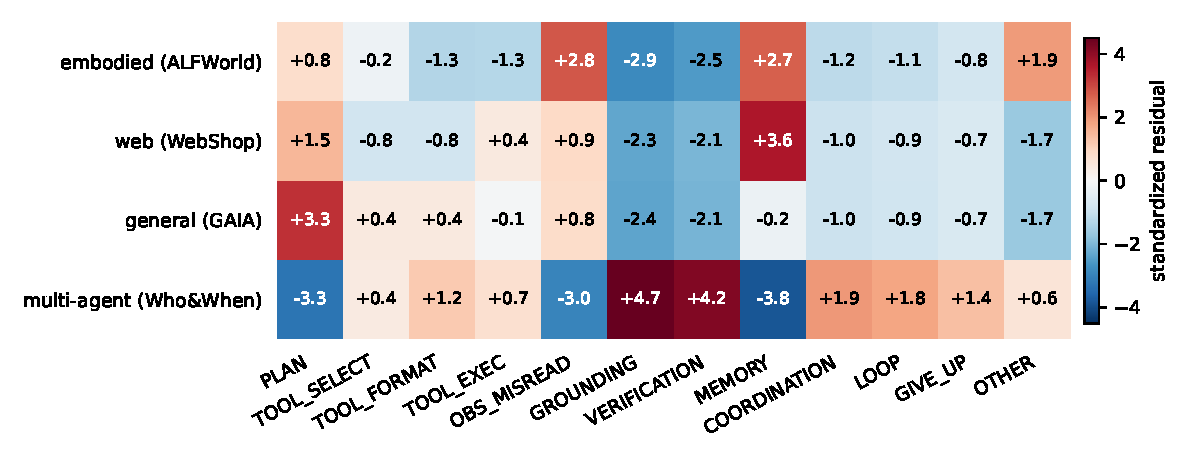
\includegraphics[width=0.95\linewidth]{figures/Figure6.pdf}
\caption{Standardized residuals of unified failure class by domain. Positive
cells are over-represented relative to independence. Residuals are
used descriptively to localize the omnibus association; individual cells
are not interpreted as separately confirmatory tests.}
\label{fig:residuals}
\end{figure}

\section{Discussion}
\label{sec:discussion}
Five implications follow. First, \textbf{harmonized failure-label
distributions differ dramatically across the public datasets studied
here}, but we cannot attribute the gap to the taxonomies alone. The two
datasets differ simultaneously in tasks, systems, and annotation protocols,
which co-vary with the label differences, so a distributional gap cannot
isolate a taxonomy effect. This audit shows that aggregate frequencies depend on benchmark context
and coding choices. Frequency differences alone neither prove nor disprove
that a category system can be applied consistently to new trajectories. Cross-paper claims of the form ``planning remains
the dominant failure mode'' are at minimum benchmark-, domain- and
model-relative, not universal. This cautions against a growing practice in
the evaluation literature~\cite{yehudai2025survey}: treating taxonomy
categories as portable measurement instruments.

Second, \textbf{benchmark label quality is a first-order problem}. A 13.5\%
empty-label rate concentrated in one model's trajectories, inconsistent
category strings, and documentation mismatches mean published failure-profile
numbers built on these files should be treated with caution until the
annotations are repaired. The field currently invests heavily in taxonomy
\emph{design}~\cite{zhu2025agentdebug,zhang2025whowhen}; our audit suggests
equal investment is needed in annotation \emph{execution and quality
control}.

Third, the \textbf{multi-agent surprise}: if coordination failures are a
characteristic failure mode of multi-agent systems, we might expect them to
be prominent in a benchmark explicitly studying multi-agent failures;
instead, grounding failures dominate here (36/184, 19.6\%); tool-formatting failures are uncommon (10/184) once bare ``code is incorrect'' reasons are coded as unmappable per the class definition (Section~\ref{sec:robustness}). This could reflect annotation focus or genuine task differences;
the present data do not distinguish those explanations.

Fourth, no released annotation in either dataset mapped to
\texttt{NO\_RECOVERY} under our coding procedure, which suggests the field's vocabulary for
``failure to recover'' outruns its measurement of it. Recovery behavior may
be the most under-instrumented dimension of agent evaluation, and benchmarks
in the ReAct tradition~\cite{yao2023react} are well placed to instrument it:
future reason--act trajectory releases could explicitly label whether
recovery was attempted and how it failed.

Fifth, \textbf{for benchmark designers}, our audit yields concrete
recommendations
\label{sec:recommendations}: (1) validate annotation pipelines per model, not just per
benchmark: our empty labels clustered in one model's trajectories;
(2) enforce a controlled vocabulary for category strings at write time
(case, spacing and naming variants silently split categories downstream);
(3) keep documentation and definition files in sync (the 17-vs-18 mismatch
is a one-line fix); (4) publish inter-annotator agreement for failure
labels, as is standard for the task labels themselves; and (5) annotate
\emph{recovery attempts}, the dimension our data suggest is most neglected.

\subsection{Guidance for agent builders}
\label{sec:builders}
Our results also carry practical lessons for practitioners choosing where to
harden agents. \emph{Match the mitigation to the domain, not to the
literature average.} An embodied agent's failure budget is dominated by
observation misreading and memory ($r{=}+2.8$, $+2.7$ in ALFWorld); invest
in perception checks and episodic state tracking before fancier planning.
A web-shopping agent fails on memory of constraints ($+3.6$ in WebShop), so
constraint-carrying context deserves the engineering effort. A
general-assistant agent fails at planning ($+3.3$ in GAIA), which is where
decomposition and verification scaffolds are the natural hypothesis to test
first. \emph{Do not assume
multi-agent means coordination risk:} in the multi-agent dataset studied
here, coordination was 3.3\% of consensus-coded failures while grounding
failures dominated, observation handling and individual tool use are candidate
interventions to evaluate before investing primarily in coordination protocols;
19.0\% of the multi-agent reasons are unmappable under the corrected coding (Section~\ref{sec:robustness}). \emph{Expect model-specific
failure signatures:} Qwen3-8B's plan-heavy profile versus GPT-4o's
memory-heavy one means a mitigation tuned on one model may not transfer to
another; evaluate failure profiles per model you ship. Finally,
\emph{instrument recovery explicitly}: no released annotation in either
dataset mapped to \texttt{NO\_RECOVERY}, so recovery behavior is unmeasured
in these datasets, and methods like Reflexion~\cite{shinn2023reflexion}
suggest structured recovery is a candidate for evaluation rather than an intervention tested here. If your evaluation logs trajectories, label the recovery
attempts; these datasets leave you flying blind on them.

\subsection{Threats to validity}
\label{sec:threats}
\emph{Construct validity:} our unified scheme inherits boundary decisions
in the analyst-defined scheme; a different scheme could shift marginal cases
(e.g., \texttt{reflection.hallucination}). We mitigate this by publishing the
full mapping with rationales and reporting scheme gaps explicitly.
\emph{Internal validity:} Who\&When codings were produced under a documented
guide and independently second-coded (agreement 69.6\%, $\kappa=0.662$,
substantial); all 56 disagreements were adjudicated to consensus labels, and
Section~\ref{sec:robustness} reports coder-specific distributions plus sensitivity analyses
showing which findings survive alternative resolutions. Residual risk is that
both coders share the guide's boundary assumptions, so the per-model analysis
stays exploratory rather than
confirmatory. \emph{External validity:} 384 failures from two datasets
cannot represent the full space of agent failures; both datasets are
English-language and researcher-curated, software-engineering agents of
the SWE-agent type~\cite{yang2024sweagent} are unrepresented, and the
recent MAST dataset~\cite{cemri2025mast} is not covered here. Moreover,
the 184 Who\&When rows contain only 139 unique question IDs (45 questions
contribute a second row each), so we re-ran the confirmatory tests with
question-level units (Section~\ref{sec:cluster}): the associations remain
significant under cluster permutation, and the grounding plurality holds in
86.7\% of cluster-bootstrap resamples when ties count. \emph{Conclusion
validity:} the original hypotheses and row-level tests were prespecified; the
revised coding, cluster checks and model stratification are retrospective
sensitivity analyses. The exploratory model
comparison is clearly marked and should be confirmed on larger, balanced
samples.

\subsection{Limitations}
\label{sec:limitations}
Beyond the threats above: the sample covers three models in only one
dataset; AgentErrorBench's empty labels reduce the effective Llama sample to
33; and our domain comparison conflates benchmark, task distribution and
annotation protocol, which co-vary in observational data. We therefore frame
the study as a descriptive audit of harmonized failure annotations, not a
controlled test of taxonomy portability: the observed gaps cannot isolate a
taxonomy effect, and the observed frequencies should not be treated as universal rates. A controlled
experiment (same tasks, same annotators, varying only the taxonomy) would
isolate the taxonomy effect, and we encourage it.

\section{Conclusions}
We audited whether agent failure taxonomies travel across datasets, by
harmonizing 384 annotated failures from two independently produced public
datasets into one 13-class scheme. The harmonized label distributions differ
dramatically across datasets, domains and models; native labels contain
nontrivial noise; and key characterizations (notably the multi-agent
grounding plurality and the 19.0\% unmappable share) are robust to the remaining coding sensitivity (Section~\ref{sec:robustness}). Because
tasks, systems, and annotation protocols co-vary across the datasets, these
gaps cannot isolate a taxonomy effect, and the observed frequencies should not be treated as universal rates. The field should report the benchmark context of failure-label frequencies
and invest in label quality with the same seriousness it invests in taxonomy
design. For practitioners, the domain narratives in Section~\ref{sec:narratives} give a
concrete starting point, framed as hypotheses to test rather than tested
prescriptions: harden perception and memory for embodied agents, constraint
tracking for web agents, planning for assistant agents, and individual tool
use for multi-agent systems. For benchmark designers,
the five recommendations in Section~\ref{sec:recommendations} are cheap to implement and would make
the next generation of failure datasets genuinely comparable. Until then,
any claim about ``how agents fail'' should come with a benchmark name
attached.

\section{Data Availability}
The annotations for 384 failures, native-to-unified mappings, original and
revised Who\&When labels, the 27-row recoding audit, the prospective analysis
plan, all analysis and resampling scripts, generated results and figure
sources are provided in Supplemental Data S1. The matching public repository
is \url{https://github.com/abhinav-TB/agent-failure-taxonomies-travel}.
Original analysis artifacts are released under the MIT license; upstream
materials retain their original terms as documented in the supplement.

\section*{Funding}
The authors received no funding for this work.

\section*{Competing Interests}
The authors declare no competing interests.

\FloatBarrier
\printbibliography

\end{document}
